% !TeX spellcheck = en_GB
\chapter{Introduction}
\label{chp:introduction}

\begin{OpeningQuote}
Network models [must] reflect the fundamental and
essential temporal nature of actual nervous systems. External processes and
events are extended in time and for a nervous system successfully to recognize
and respond may require temporally extended representation; movements required for behavior involve sets of bodily motions sequenced in time; short-term memory is a trick for allowing present access to the recent past, and
longer-term memory to the more remote past.
\OpeningQuoteSource{Particia S. Churchland and Terrence J. Sejnowski}{The Computational Brain (1992)}
\end{OpeningQuote}


Biological neural networks are dynamical systems.
Of course, taken at face value, this is quite an understatement---just like all physical systems, biological systems evolve through time and are thus \enquote{dynamic}.
However, dynamics are of paramount interest when studying the brain (\cite{churchland1992computational}, Section 3.9).
At the lowest level, dynamics shape computation within individual neurons and dendritic structures.
Simultaneously, at the highest level, dynamics determine the ability of an organism to survive.
Variations in response-time on the order of milliseconds can make the difference between life and death, as avid viewers of nature documentaries and operators of motor vehicles will surely attest.

From the perspective of computer engineering it seems almost implausible that biological systems should be capable of rapid coordinated action---especially considering that the elements that make up nervous systems compute asynchronously and possess strong intrinsic dynamics.
After all, when constructing artificial computers, asynchronicity and dynamics are mere annoyances of physical reality that engineers seek to eliminate.
Typical microprocessors spend a sizeable portion of their energy budget on distributing clock signals \citep[e.g.,][]{zhang2008injectionlocked}, and digital circuits are meticulously designed to switch between clearly interpretable voltage states as quickly as possible \citep[e.g.,][Chapter~4]{weste2011cmos}.
Similarly, on an algorithmic level, computer scientists assume that neurons in artificial neural networks compute instantaneously, while time progresses in discrete, synchronous steps \citep[e.g.,][Chapter~10]{goodfellow2016deep}.

This juxtaposition of artificial and biological systems gives rise to an old, but still common (and rather subtle) mis\-cha\-rac\-te\-ri\-sa\-tion---namely, the idea that biological information processing is slow and that, compared to digital computers, biological brains compensate for their slowness with massive parallelism (e.g., \cite{vonneumann1958computer}, pp.~50f).
There is, for sure, a kernel of truth to this statement.
For example, signal propagation in electronic circuits is between six and eight orders of magnitudes faster than axonal action potential propagation.%
\footnote{Electrical signals travel at about two thirds of the speed of light along conductors (i.e., about \SI{200e6}{\metre\per\second}). Axonal action potential propagation reaches between \SIrange{1}{100}{\metre\per\second} \citep[Chapter~2, p.~23]{kandel2012principles}.}
Still, stating that neurons and synapses are \enquote{slow} is misleading at best.
On the one hand, neural \emph{networks} can be much faster than their slowest elements (cf.~\Cref{fig:ff_vs_rec_response_time}), and, on the other hand, the \enquote{slow} neural dynamics are an \emph{intrinsic} part of the computation that is being performed.
Put differently, and rephrasing the above \Citeauthor{churchland1992computational} quote, computation that depends on the history of a signal on short time-scales is possible \emph{because} information about the past is implicitly retained by the \enquote{slow} temporal dynamics, and not \emph{despite} this fact.

\begin{figure}[p]
	\centering
	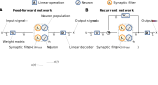
\includegraphics{media/chapters/01_introduction/ff_vs_rec_response_time_overlay.pdf}%
	\kern-158mm\includegraphics{media/chapters/01_introduction/ff_vs_rec_response_time.pdf}
	\caption[Neural networks can be faster than their fastest time-constant]{Neural networks can be faster than their fastest feed-forward time-constant. See \Cref{sec:nef,sec:temporal_tuning_lti} for more information.
	\textbf{(A)} Feed-forward computation with \SI{100}{\milli\second} first-order low-pass filters (\emph{synaptic filters}) in its forward path. Sending a pulse signal $u(t)$ into this network, we receive a low-pass filtered output $x(t)$ that \emph{slowly} converges to $u(t)$.
	\textbf{(B)} By adding recurrent connections and solving for weight matrices $\mat W$, $\mat W_\mathrm{rec}$, we can (in the limit of $n \to \infty$) realise any dynamical system, including low-pass filters with time-constants $\tau' < \tau$ (coloured lines;  cf.~\cite[Chapter~8]{eliasmith2003neural}).
	}
	\label{fig:ff_vs_rec_response_time}
\end{figure}

\begin{table}[p]
	\small\sffamily
	\centering
	\caption[Comparison between spatial and spatiotemporal computation]{Comparison between spatial and spatiotemporal computation. Spatial (static, or non-temporal) computation can be modelled as a first-order functions $f$, spatiotemporal computation relies on second-order functions processing the entire input history $\mathfrak{x}(t)$ for $t \leq 0$.
	Listed are the resources used to establish the function basis, i.e., tuning curves, in neural networks (see also \Cref{chp:temporal_tuning}).
	}
	\label{tbl:spatiotemporal}
	\begin{tabular}{r p{5.9cm} p{5.9cm}}
		\toprule
		& \textbf{Spatial computation} & \textbf{Spatiotemporal computation} \\
		\cmidrule(l){2-2}\cmidrule(l){3-3}
		&  $\begin{aligned} f: \mathbb{R}^d &\longrightarrow \mathbb{R}^{d'} \\ f(\vec x) &\mapsto \vec y \end{aligned}$ & $\begin{aligned} f : (\mathbb{R}^- \longrightarrow \mathbb{R}^d) &\longrightarrow \mathbb{R}^{d'} \\ f(\mathfrak{x}) &\mapsto \vec y\end{aligned}$ \\
		\cmidrule{1-1}\cmidrule(l){2-2}\cmidrule(l){3-3}
		\textit{Domain} & Input $\vec x \in \mathbb{R}^d$ & Signal $\mathfrak{x} \in \{ f \mid f : \mathbb{R}^- \longrightarrow \mathbb{R}^d) \}$ \\
		\cmidrule{1-1}\cmidrule(l){2-2}\cmidrule(l){3-3}
		\textit{Codomain} & Output $\vec y \in \mathbb{R}^{d'}$ & Output $\vec y \in \mathbb{R}^{d'}$ \\
		\cmidrule{1-1}\cmidrule(l){2-2}\cmidrule(l){3-3}
		\textit{Function basis} & Tuning curves $a_i(\vec x)$ & Temporal tuning curves $a_i(\mathfrak{x})$ \\
		\cmidrule{1-1}\cmidrule(l){2-2}\cmidrule(l){3-3}
		\textit{Neural resources}  & \textbullet\ Somatic \& dendritic nonlinearities & \textbullet\ Somatic \& dendritic nonlinearities \\
		                  & & \textbullet\ Synaptic filters \& axonal delays \\
		                  & & \textbullet\ Intrinsic dynamics \\
		                  & & \textbullet\ Recurrent connections \\
		\bottomrule
	\end{tabular}
\end{table}

While it is undisputed that dynamics play an important role in the brain, there are few \emph{overarching} theories that suggest how dynamics should be integrated into models of biological and cognitive systems.
Cybernetics \citep{wiener1948cybernetics} and dynamicism \citep{vangelder1998dynamical,eliasmith1996third} stand out as attempts to establish dynamics-focused research programs, but, as of writing, have either been subsumed by other fields or faded to obscurity.
Instead, the temporal evolution of biological and cognitive systems are modelled, often separately, at every possible level of abstraction---from individual neurons and their subcomponents \citep[e.g.,][]{gerstner2002spiking,izhikevich2007dynamical}, over small- and large-scale networks \citep[e.g.,][]{gerstner2014neuronal,bassett2017network}, to behaviour and language \citep[e.g.,][]{anderson1997actr,debot2007dynamic}.

What is missing are \emph{bridging laws}, that describe in broad strokes how low-level mechanism gives rise to high-level behaviour and cognition.
Building upon earlier work by \citet{eliasmith2003neural}, this thesis is an attempt at providing such laws.

In particular, our goal is to study ways in which low-level neural dynamics can be harnessed as a resource for high-level function.
We approach this from two different directions.
First, we analyse the dynamics intrinsic to passive dendritic trees, and derive a static model of dendritic nonlinearity that can be systematically exploited for high-level, non-temporal computation.
Second, we investigate \enquote{temporal tuning} as a low-level characterisation of individual model neurons.
This allows us to construct networks that can approximate arbitrary spatiotemporal functions (cf.~\Cref{tbl:spatiotemporal}), while outperforming common methods from machine learning.

Importantly, we focus on being as integrative as possible.
That is, our goal is \emph{not} to model biological phenomena at the greatest possible detail, but to think about mathematically tractable ways in which a broad range of neurophysiological and behavioural phenomena can be captured.
This way, we hope to provide a useful tool for researchers wishing to model high-level function, while constraining their work to physiological data.

Similarly important, and returning to our comparison between brains and computers, our approach is not only useful for cognitive modellers, but also for scientists working on brain-inspired computers (so called \emph{neuromorphic hardware}), and to the field of machine learning.
Systematically thinking about ways in which the computational substrate connects to function informs both the architecture of neuromorphic computers, and suggests a \enquote{neural compiler} for realising desired algorithms on these devices \citep{boahen2017neuromorph,voelker2021programming}.
Furthermore, our approach lends itself to thinking about the \enquote{best possible} representation that should be established in a neural network, and can thus pave the way for artificial neural networks that are faster to train, more data-efficient, and higher performing \citep{voelker2019lmu,chilkuri2021parallelizing}.

\subsubsection{Structure and overview of this thesis}

The remainder of this thesis is structured as follows.
In \Cref{chp:modelling_neurobiological_systems} we review the aforementioned techniques for modelling and simulating neurobiological systems.
For readers with a mathematical, but no further biology background, we first introduce fundamental concepts from neuroscience, and then discuss our main modelling technique, the \emph{Neural Engineering Framework} (\NEF; \cite{eliasmith2003neural}).
We close with a discussion of shortcomings of the \NEF that we hope to resolve in this thesis.

We continue in \Cref{chp:nlif} by describing novel methods for integrating complex neuron models with multiple input channels and conductance-based synapses into \NEF networks.
Specifically, we focus on a mathematically tractable extension to the \LIF neuron, namely the $n$-compartment \LIF, or \nlif, neuron.
The purpose of this is twofold.
First, our extensions to the \NEF allow modellers to better constrain their models to neurophysiological data (we explore this in more detail in \Cref{chp:cerebellum}).
Second, we demonstrate---both in theory, and in simulation---that it is possible to systematically exploit the dynamics intrinsic to the passive dendritic tree of the \nlif neuron to perform multivariate, non-temporal computation in a spiking neural network context.
That is, \NEF networks with \nlif neurons can be made to automatically employ a simple form of \emph{dendritic computation} \citep{mel1994information,london2005dendritic} and to thus approximate a larger range of functions well compared to similar networks with standard \LIF neurons, sometimes outperforming two-layer networks.
In particular, we can model gain modulation, an important phenomenon in the central nervous system \citep{salinas2000gain,chance2002gain}.
Our results may inform the design of future neuromorphic hardware and enable a better utilisation of existing neuromorphic computers.

Next, in \Cref{chp:temporal_tuning}, we introduce the notion of \emph{temporal tuning curves} to the \NEF.
Based on a model of spatiotemporal receptive fields in visual cortex \citep{carandini1999linearity}, temporal tuning curves provide a systematic way to compute functions \emph{through time} (\Cref{tbl:spatiotemporal}).
This approach is a generalisation of the \NEF dynamics principle, and a paradigm shift that offers a unified view onto resources for temporal computation, including synaptic filters, time-delays, and, to some degree, intrinsic neural dynamics.

Interestingly, we can, with small modifications, reuse a convex optimisation problem derived in the previous chapter to solve for weights that realise desired temporal tuning.
The weight solving procedure does not distinguish between feed-forward and feedback connections, and we can employ feedback connections to realise diverse temporal tuning.
Building upon previous work by \citet{voelker2018improving}, we show that mapping linear time-invariant (\LTI) systems approximating sliding-window transformations onto spiking neural networks generates temporal tuning that resembles time cells \citep{pastalkova2008internally,howard2014unified,tiganj2016sequential}.
We present a general method for constructing such \LTI systems.

Interestingly, our spatiotemporal \NEF populations are equivalent to a layer of Legendre Memory Units (\LMUpl; \cite{voelker2019lmu}).
\LMUpl are an exciting artificial neural network architecture for stream-to-stream processing.
We find evidence that one of our \LTI systems may possess more favourable computational properties compared to the standard \LTI system used in the \LMU, while offering a higher performance in some experiments.

As a final experiment in \Cref{chp:cerebellum}, we combine the approaches outlined in the previous chapters to construct an adaptive filter model of the cerebellum \citep{fujita1982adaptive}.
We apply our methods for building \NEF networks with more biological constraints (including Dale's principle; cf.~\Cref{chp:nlif}) in the context of the recurrent Granule-Golgi circuit.
This circuit can in principle implement an \LTI system generating a temporal basis as discussed in \Cref{chp:temporal_tuning}.
Building upon the Granule-Golgi circuit we constrcut a network that can learn to decode arbitrary delays, reproducing basic features of eyeblink conditioning \citep[e.g.,][]{heiney2014cerebellardependent}.

We conclude with a short discussion of our contributions and potential future work in \Cref{chp:conclusion}.
Proofs and additional information may be found in \Cref{app:math_detail,app:data}, and an overview the software written for this thesis, namely \emph{libnlif} and \emph{NengoBio} in \Cref{app:software}.

\begin{FloatingBox}{Notation}
\setlength{\parskip}{0.5em}
%Some effort has been made to be as consistent as possible in the mathematical notation.
Bold lower-case letters (e.g., $\vec x$, $\vec \gamma$) denote vectors, while bold upper-case letters (e.g., $\mat X$, $\mat \Gamma$) denote matrices.
Double-struck letters denote sets, with $\mathbb{N}$, $\mathbb{Z}$, $\mathbb{Q}$, $\mathbb{R}$, $\mathbb{C}$ being our usual number systems.
$\mathbb{R}^+$ and $\mathbb{R}^-$ are the positive and negative real numbers (including zero).

We generally assume that vectors are column vectors, i.e., $\vec x \in \mathbb{R}^d$ is implicitly a matrix $\vec x \in \mathbb{R}^{d \times 1}$.
Correspondingly, $\vec x^T \vec y =  \langle \vec x, \vec y \rangle$ forms an inner product, and $\vec x \vec y^T = \vec x \otimes \vec y$ is an outer product.

When describing an entry in the $i$th row and the $j$th column of a matrix $\mat M$, we write $( \mat M )_{ij}$; $(\mat M)_i$ corresponds to the $i$th row, whereas $(\mat M^T)_j$ corresponds to the $j$th column.
All indices start with one.

We use the standard notation for the $L^p$ vector norm and the Frobenius matrix norm. Let $\vec x = (x_1, \ldots, x_d)$ and $\mat M \in \mathbb{R}^{m \times n}$ with $(\mat M)_{ij} = m_{ij}$. Then
\begin{align*}
	\|\vec x\|_0 &= | \{ x_k | x_k \neq 0 \} | \,, & 
	\|\vec x\|_p &= \sqrt[p\,\,]{\sum\nolimits_{k=1}^d |x_k|^p } \,, &
	\|\vec x\|_\infty &= \max\{ x_1, \ldots, x_d\} \,, &
	\| \mat M \|_\mathrm{F} = \sqrt{\sum\nolimits_{i=1}^m \sum\nolimits_{j=1}^n m_{ij}^2} \,\,.
\end{align*}
We define the inner product $\langle f, g \rangle$ and the convolution $f \ast g$ of two functions $f, g : \mathbb{R} \longrightarrow \mathbb{R}$ as
\begin{align*}
	\langle f, g \rangle &= \int_{-\infty}^\infty f(\tau) g(\tau) \,\mathrm{d}{\tau} \,, & 
	(f \ast g)(t) &= \int_{-\infty}^\infty f(t - \tau) g(\tau) \,\mathrm{d}{\tau} \,.
\end{align*}
\end{FloatingBox}
